\chapter{Introdução} \label{cap:intro}
Atualmente, o aprendizado de máquina permeia o cotidiano humano
provendo auxílio em tarefas diversas.
\ano{citar algumas(gps,digitação,fala))? precisa de ref?}
Seu bom desempenho, na tarefa de classificação, depende da existência de:
\begin{itemize}
 \item \textbf{amostragem} de dados de qualidade para construção de um acervo \ano{acervo?};
 \item um processo de \textbf{categorização} desses dados que exponha conhecimento
 suficiente para a tarefa desejada; e,
 \item um algoritmo de \textbf{aprendizado} adequado.
\end{itemize}
Enquanto a \textit{categorização} dos dados é normalmente
realizada por um supervisor humano que atribui categorias/classes para cada objeto/exemplo
de interesse contido nos dados,
a forma de \textit{amostragem} de exemplos
e a determinação do algoritmo de \textit{aprendizado} dependem de
um segundo especialista,
com conhecimento específico da área de aprendizado de máquina.

\ano{citar problemas? fadiga ...}

O segundo especialista pode resolver o problema da escolha do algoritmo
recorrendo à sua experiência pessoal ou adotando algum sistema automático de
recomendação como o \textit{meta-aprendizado} conforme descrito no
Capítulo \ref{meta}.
Ambas as abordagens, manual e automática,
são aplicáveis apenas no cenário em que o acervo, chamado de conjunto de treinamento,
já está construído.
Consequentemente, a escolha do processo de amostragem,
denominado \textit{aprendizado ativo},
precede a determinação do algoritmo de aprendizado.
\ano{isso contradiz o cenário em que o aprendiz é definido de antemão,
que é parte dos experimentos}

Da mesma forma que existe o problema da escolha do algoritmo de aprendizado
mais apropriado, existe o problema da escolha da melhor estratégia de
aprendizado ativo.
O segundo problema é mais complexo, tendo-se em vista que o sucesso
da estratégia escolhida só pode ser determinado após ter-se incorrido
em custos financeiros com a atividade de supervisão - que é realizada
frequentemente por um humano, chamado genericamente de \textit{oráculo}.
% Está implícita na seleção de dados de qualidade a economia em tempo de processamento e
% de supervisão, dado que apenas a parcela reduzida de exemplos mais relevantes
% é enviada para a análise do oráculo e processada pelo algoritmo de aprendizado.
% Como agravante, a quantidade global de dados duplica a cada dois anos
% \citep{journals/sigkdd/ZliobaiteBGGGMM12}, apontando
% para uma tendência que torna intratável a supervisão e aprendizado exaustivos
% em muitas aplicações.
% 
% Por outro lado, aplicações em que o oráculo é um processo químico, por exemplo,
% envolvem consumo de material ou a destruição dos exemplos consultados.
% Apesar de não envolver a manutenção dispendiosa de um oráculo humano
% e possivelmente não requerer uma filtragem massiva de exemplos,
% cada consulta tem um custo associado.
Dessa forma, é preciso adotar uma estratégia
com base em previsões de desempenho ou de acordo com características da base
de dados.
Na prática, essa escolha tem sido quase arbitrária, tendendo a se concentrar
no uso da estratégia mais simples (amostragem por incerteza).
Essa preferência foi reportada numa competição de aprendizado ativo,
onde também prevaleceu a ausência de estratégias possivelmente mais efetivas
como as baseadas em densidade conforme
Figura \ref{compet}.
\ano{é mesmo mais efetiva? por quê?}
\begin{figure}
\caption{Frequência de uso de estratégias na competição de aprendizado ativo
(alguns participantes adotaram mais de uma estratégia).
\textit{Adaptado de \citep{journals/jmlr/GuyonCDL11}.}}
\label{compet}
\begin{center}
    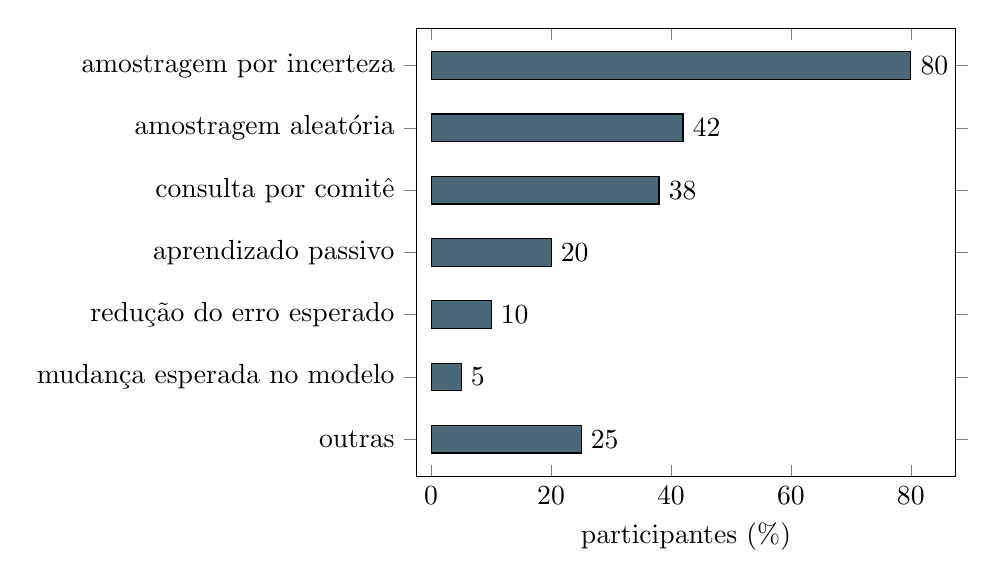
\begin{tikzpicture}
\begin{axis}[
    xbar,
%     xmin=0.0,
%     width=12cm,
%     height=40cm,
%     enlarge x limits={rel=0.13,upper},
    ytick={1,2,3,4,5,6,7},
    yticklabels={
    {amostragem por incerteza},
    {amostragem aleatória},
    {consulta por comitê},
    {aprendizado passivo},
    {redução do erro esperado},
    {mudança esperada no modelo},
    {outras}
    },
%         enlarge y limits=0.4,
    xlabel={participantes (\%)},
    ytick=data,
    nodes near coords,
    nodes near coords align=horizontal
]
\addplot [draw=black, fill=cyan!40!black] coordinates {
    (80,7)
    (42,6)
    (38,5)
    (20,4)
    (10,3)
    (5,2)
    (25,1)
};
\end{axis}
\end{tikzpicture}
\end{center}
\end{figure}

% challenge:
% global_score = (ALC-Arand)/(Amax-Arand)       Amax = 1
% semi-supervised learning is needed to achieve good performance in the first part of the learning curve
% (usar ou não semisupervised é um problema à parte, que faz parter do learner, não da estratégia; classificadores semisupervisionados são melhores, mas não é isso que se está avaliando quando se comparam estratégias; ensembles, feature selection e SMOTE também ajudam e nem por isso precisam ser empregados na comparação de estratégias)


Em consonância com esse panorama,
está a ausência de estudos comparativos
abrangentes que possam guiar o especialista na fase de amostragem.
% - até onde o conhecimento do autor permite dizer - 
\ano{AL é uma área com enfoque prático, pois visa diretamente a redução de custos.
Provavelmente por esse motivo, a pesquisa em AL é normalmente direcionada a
aplicações específicas e não a experimentos comparativos abrangentes.}


\esb{comenta possiveis deficiencias ou
lacunas das estrategias existentes (pensando nas que vou propor),
apresenta melhorias propostas;
apresenta recomendação de classificador e/ou estratégia;
apresenta hipóteses principal e secundárias.
Falar ainda dos objetivos da tese, que estao bem ligados as hipoteses}

Hipóteses secundárias
Estratégias baseadas em densidade são viáveis \ano{muito fraca essa palavra?} sem um aprendiz
objetivo: contornar o problema de escolha do algoritmo de aprendizado antes
da obtenção dos rótulos (transformando uma estratégia eficaz em agnóstica)

É possível definir a estratégia mais adequada \ano{muito forte essas duas palavras?} por meio de recomendação automática
objetivo: resolver o problema de escolha da estratégia quando o algoritmo de
aprendizado é dado previamente pela aplicação (com recomendação automática)




\section{Contribuição}\label{contribuicao}
\esb{cita os artigos/software publicados e submetidos; menciona
metodologia, compara com Everton e de que forma organiza a área}

\section{Cenário}\label{cenario}
Existem três principais cenários na literatura de aprendizado ativo
\citep{settles2010active}:
\textit{síntese de consulta por associação} ou
\ing{consulta de exemplos sintetizados}{membership query synthesis};
\ing{amostragem baseada em \pool}{pool-based sampling}; e
\ing{amostragem seletiva baseada em fluxo}{stream-based selective sampling}.
Mais detalhes são apresentados no Apêndice \ref{cenarios}.
O cenário adotado neste trabalho é baseado em \pool.
Especificamente, há as seguintes restrições de escopo:
\begin{itemize}
 \item consulta pela classe (não por valores de atributos, por exemplo);
 \item monorrótulo;
 \item distribuição estacionária;
 \item custo por erro de classificação uniforme;
 \item custo por consulta uniforme;
 \item oráculo único e constante sujeito a ruído;
 \item os domínios dos atributos nominais são previamente conhecidos;
 \item atributos sem valores faltantes;
 \item consulta \ing{um a um}{on-line}.
\end{itemize}

\section{Estrutura do documento}\label{estrutura}
O contexto da pesquisa, a notação matemática e a terminologia adotadas e a revisão da literatura das áreas
envolvidas neste trabalho são apresentados no Capítulo \ref{contexto}.
No Capítulo \ref{propostas},
são apresentadas as propostas de algoritmos.
O Capítulo \ref{metodologia} contém os métodos de avaliação e detalhes de
implementação comuns a todos os experimentos descritos neste documento.
Essa avaliação empírica e seus resultados associados são apresentados
no Capítulo \ref{experimentos}.
Adicionalmente, uma abordagem baseada em meta-aprendizado
é proposta e avaliada no Capítulo \ref{aml}.
Por fim, uma análise geral unificada das contribuições da tese e
desdobramentos futuros são apresentados no
Capítulo \ref{conclusao}.
Detalhes sobre os cenários de aprendizado ativo, resultados,
formatação, estilo e terminologia podem ser encontrados nos apêndices \ano{ <- revisar}.

\ano{mencionar apendice de rev. sistemática? outros aps?}

%
% No Capítulo \ref{cap:classificacao}, é apresentada a notação utilizada neste trabalho juntamente com um texto introdutório sobre aprendizado supervisionado para contextualizar as duas revisões bibliográficas que o seguem: a primeira sobre \textit{ensembles} e a segunda sobre \textit{fluxos de dados}.
% Ao final, \textit{ensembles} voltados especificamente a fluxos de dados são revisados.
%
% No Capítulo \ref{cap:aprendizado-ativo}, o \textit{aprendizado ativo} é descrito em detalhes a respeito dos cenários mais comuns e das estratégias normalmente adotadas.
% Os trabalhos recentes nos quais se baseia diretamente a linha investigativa adotada são explicitados na Seção \ref{sec:panorama}.
%
% O plano de trabalho é apresentado no Capítulo \ref{cap:plano} e contempla a situação atual do aluno no programa de doutorado, os recursos disponíveis, as hipóteses formuladas, a metodologia e o cronograma.
%
% Finalmente, no Capítulo \ref{cap:experimentos}, são mostrados experimentos ilustrativos da mudança de conceito e da diversidade de comportamento entre diferentes classificadores.
